\documentclass{memoria}


\begin{document}

\portada{Informe Entrega 3: Diseño Detallado}{Gerson Aguirre Pavez\\Max Chacón Villanueva\\Daniel Gacitúa Vásquez\\Elías González Marincovic\\Nicolás Rozas Sepúlveda}{\textbf{Profesores:}\\Mauricio Marín Caihuán\\Rodrigo Vásquez Fernández\\\textbf{Ayudante:\\}José Orellana}{\today}


\indices

\capitulonn{INTRODUCCIÓN.}



%-------------------------------------------------------------------------------------
\capitulo{MARCO TEÓRICO.}

\seccion{DIAGRAMA DE CASOS DE USO.}



\seccion{DIAGRAMAS DE SECUENCIA.}



%-------------------------------------------------------------------------------------
\capitulo{DIAGRAMA DE CLASES DE DISEÑO.}

\seccion{DIAGRAMA JAVAEE.}

\figura{Diagrama de Clases JavaEE (MVC).}{
	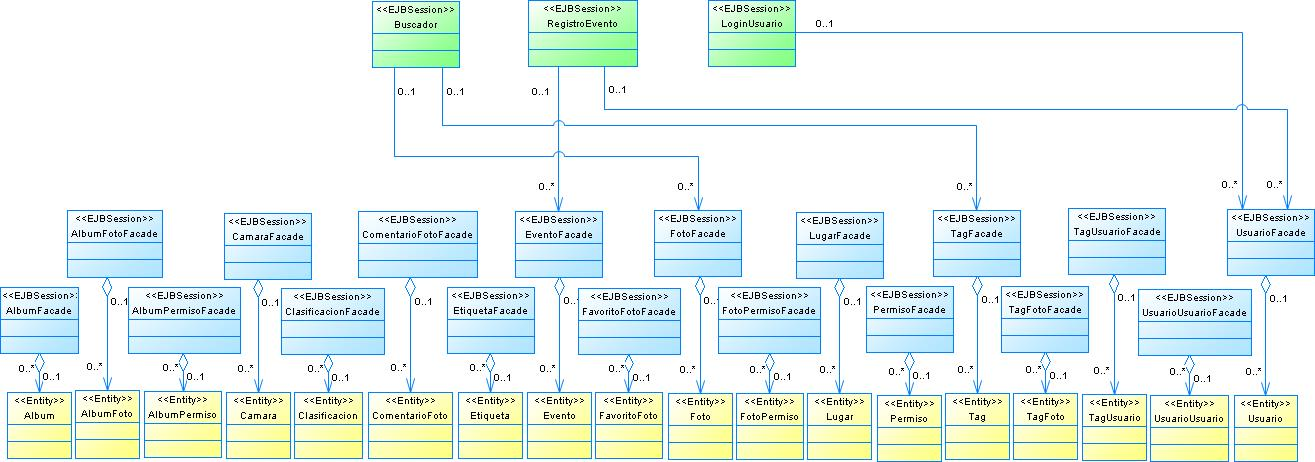
\includegraphics[width=16cm]{DiagramaModeloControlador.jpg}
}


\figura{Diagrama de Clases JavaEE (Entities).}{
	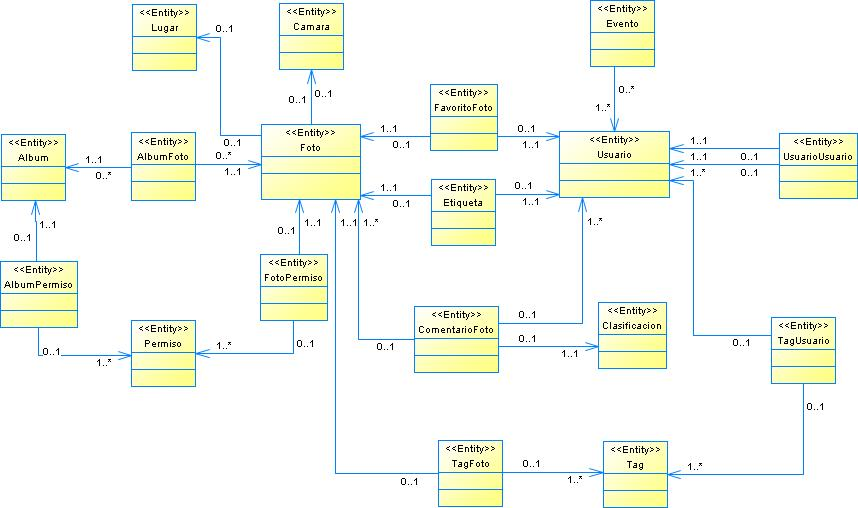
\includegraphics[width=16.5cm]{DiagramaEntities.jpg}
}

\figura{Diagrama de Clases JavaEE (Entities), parte 1.}{
	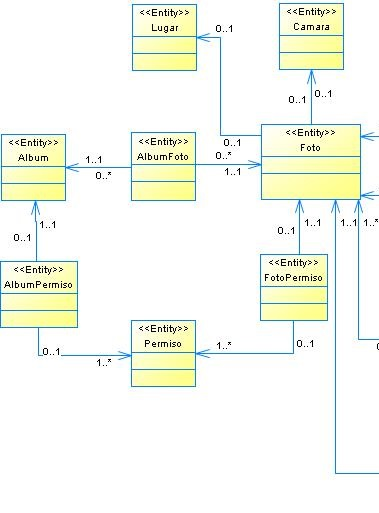
\includegraphics[width=14cm]{DiagramaEntitiesParte1.jpg}
}

\figura{Diagrama de Clases JavaEE (Entities, parte 2).}{
	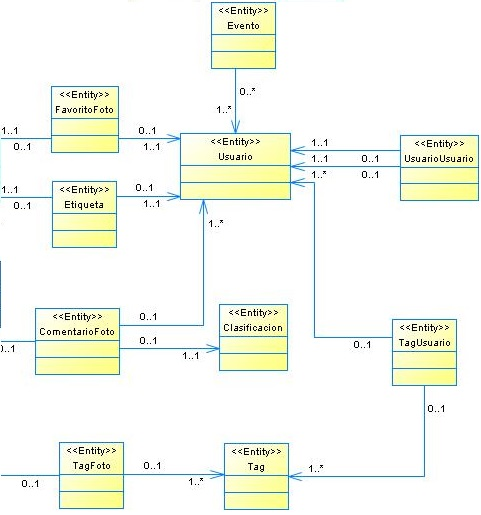
\includegraphics[width=15cm]{DiagramaEntitiesParte2.jpg}
}

\newpage
\seccion{DIAGRAMA WEB-APP (ANGULAR JS).}

\figura{Diagrama de Clases Angular JS.}{
	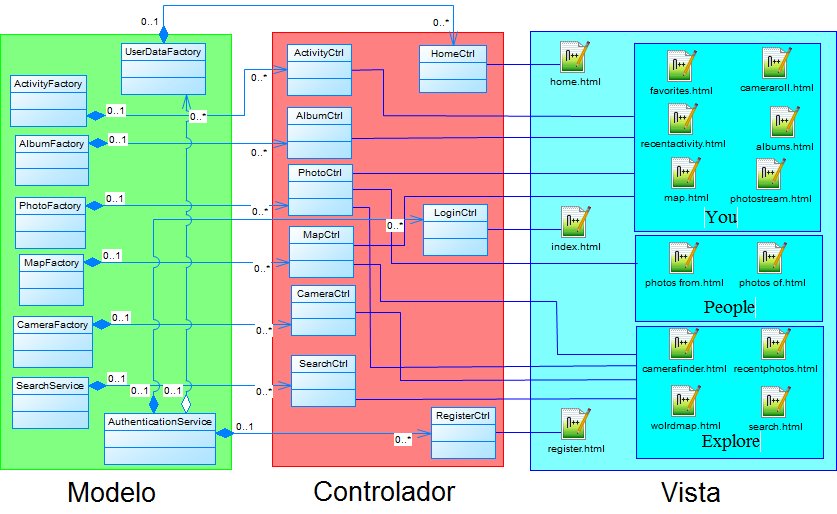
\includegraphics[width=18.5cm]{DiagramaClasesAngularJS.png}
}

El diagrama de clases en \textsl{AngularJS} tiene ciertas particularidades. Primero que todo, el diagrama está fuertemente influenciado por la Arquitectura \textsl{MVC} (Modelo-Vista-Controlador), además las estructuras de código en \textsl{AngularJS} no son clases en sí mismas, sino que son módulos que pueden cumplir diferentes propósitos según son definidos.

Dentro de los tipos de módulos tenemos los Controladores (encargados de intermediar las interacciones entre Modelo y Vista), las Factorías (encargadas de ofrecer objetos Javascript a través de funciones implementables) y los Servicios (encargados de recibir peticiones y procesarlas con la capa de Negocio).

Las Factorías y Servicios viven en la capa de Modelo, los Controladores viven en su capa homónima y los archivos HTML residen en la capa de Vista.

Cada vista HTML tiene un Controlador asignado, y cada Controlador puede llamar a una o más Factorías y Servicios, como se ve en la Figura del diagrama de clases de AngularJS.

La disposición de las clases está estrictamente ligado e impuesto por la arquitectura, en este sentido es una ventaja, ya que simplifica la tarea del diseño arquitectural a nivel de Aplicación Web.

\newpage
\seccion{DIAGRAMA LUCENE.}

El diagrama de clases mostrado en la figura 2-6, representa las principales clases que se utilizarán durante el desarrollo del buscador con la tecnología \textsl{Lucene}. Cabe mencionar que existen otras clases propias de la tecnología pero que para esta ocasión serán obviadas y solo se explicarán las principales y más características, tomando en cuenta que a medida que avance el proceso de implementación se puede utilizar muchas más clases.

\figura{Diagrama de Clases Lucene.}{	
	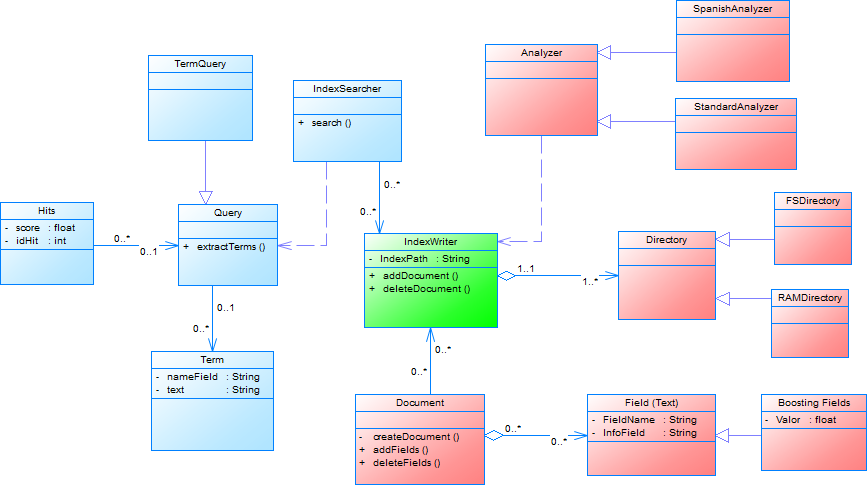
\includegraphics[width=17cm]{DiagramaClasesLucene.png}
}

Para comenzar, se muestra en la figura 2-7 la sección derecha del diagrama de la figura 2-6 que corresponde a las clases utilizadas en el proceso de indexación de \textsl{Lucene}. 

La clase \textsl{IndexWriter} (destacada con color verde en el diagrama) es la clase encargada de crear la estructura del índice invertido para realizar todas las búsquedas correspondientes. Se necesita de una clase \textsl{Analyzer}, con la que se analizarán los textos sobre los que se construirá el índice, dentro de esta clase, existen múltiples subclases de analizadores con distintos filtros, dentro de las cuales se encuentran las que se especificaron en el diagrama: \textsl{SpanishAnalyzer} y \textsl{StandardAnalyzer}, donde el primero sirve para trabajar con el lenguaje español, y el segundo se encarga de transformar todo a letra minúscula, de eliminar las \textsl{StopWords} y de aceptar caracteres especiales como acrónimos, alfanuméricos, entre otros.

Luego, se tiene una clase \textsl{Directory}, que es la encargada de almacenar el índice invertido que se ha creado. Dentro de esta clase se pueden encontrar dos subclases principales: \textsl{FSDirectory} y \textsl{RAMDirectory}. La primera, se encarga de almacenar el índice de manera física, es decir, se reserva un espacio de memoria en el disco duro donde se almacenará la estructura de datos, mientras que con \textsl{RAMDirectory} se almacena en memoria RAM para acceder de manera más rápida, luego de terminar los procesos de búsqueda, los índices en RAM se destruyen, no así los almacenados con la clase \textsl{FSDirectory}. 

\figura{Diagrama de Clases Lucene, parte 1.}{
	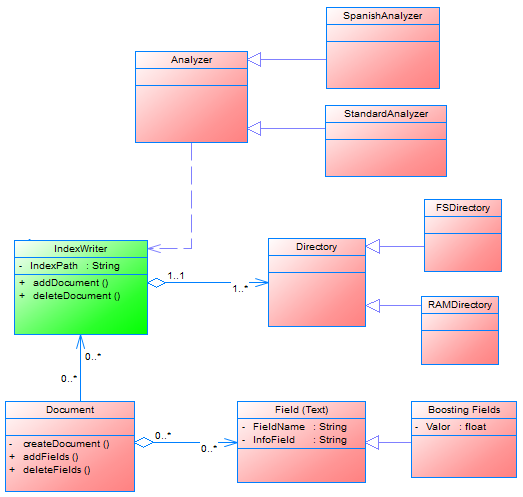
\includegraphics[width=15cm]{DiagramaClasesLuceneParte1.png}
}

Con la clase \textsl{Document}, se crean los diferentes documentos que contendrá el índice invertido, para esto, se utiliza la clase \textsl{Field}, que son los distintos campos que conformarán un documento. Cada campo, se clasifica de una manera diferente para establecer los valores que tendrán al momento de hacer una búsqueda, en este caso, se utilizará el campo \textsl{BoostingFields}, que indexarán los distintos campos asignándoles diferentes valores.
    
\newpage
\figura{Diagrama de Clases Lucene, parte 2.}{
	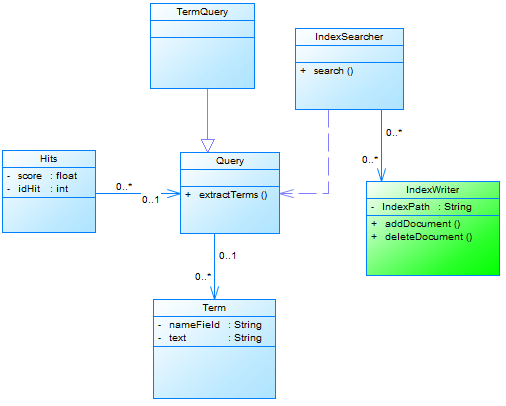
\includegraphics[width=15cm]{DiagramaClasesLuceneParte2.png}
}

Continuando con la sección izquierda del diagrama de clases, se pueden observar las clases que se utilizan para el proceso de búsqueda de \textsl{Lucene}. En primer lugar, se encuentra la clase \textsl{IndexSearcher} que se encarga de generar las búsquedas, encontrando los distintos índices invertidos (generados con \textsl{IndexWriter}) que participarán en una búsqueda específica. Dicha clase necesita de \textsl{Query}, que será la clase que realiza la consulta generada para encontrar los resultados esperados. Esta clase cuenta con varias subclases, entre ellas \textsl{TermQuery}, que es el \textsl{query} más básico y se usa para encontrar documentos con campos con valores específicos. La búsqueda como tal, debe utilizar la clase \textsl{Term}, que es la unidad básica para la búsqueda, conteniendo el nombre del \textsl{field} y el valor que se le asigna (con la clase \textsl{Boosting Fields} explicada anteriormente). Y por último, se encuentra la clase \textsl{Hit}, en donde se almacenarán todos los resultados de documentos encontrados relacionados con la búsqueda del \textsl{Query}. 

\newpage
\seccion{DIAGRAMA ANDROID.}

\figura{Diagrama de Clases Android.}{
	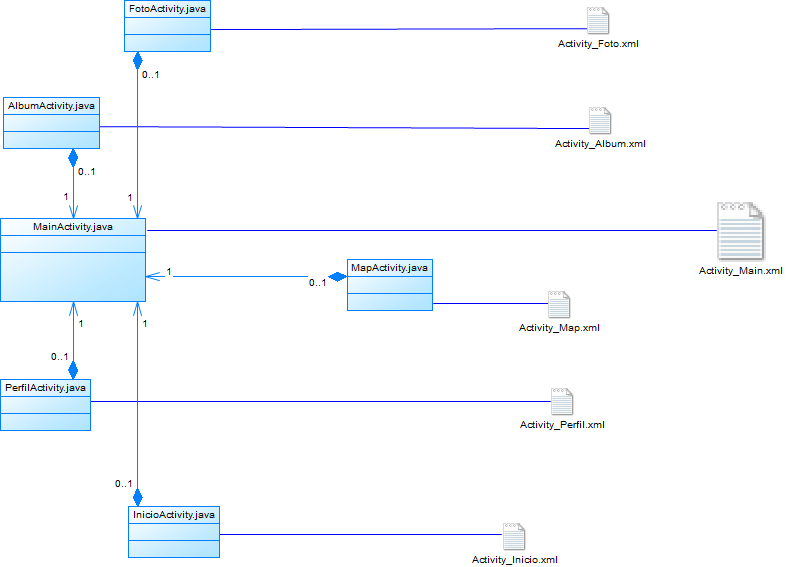
\includegraphics[width=18cm]{DiagramaClasesAndroid.png}
}
 

%-------------------------------------------------------------------------------------
\capitulo{CASOS DE USO.}

A continuación, se detallan todos los casos de uso que se especificaron en una entrega anterior (Entrega 1: Ingeniería de Requerimientos), donde se desarrolló el siguiente diagrama:

\figura{Diagrama de Casos de Uso (Ingeniería de Requerimientos.}{
	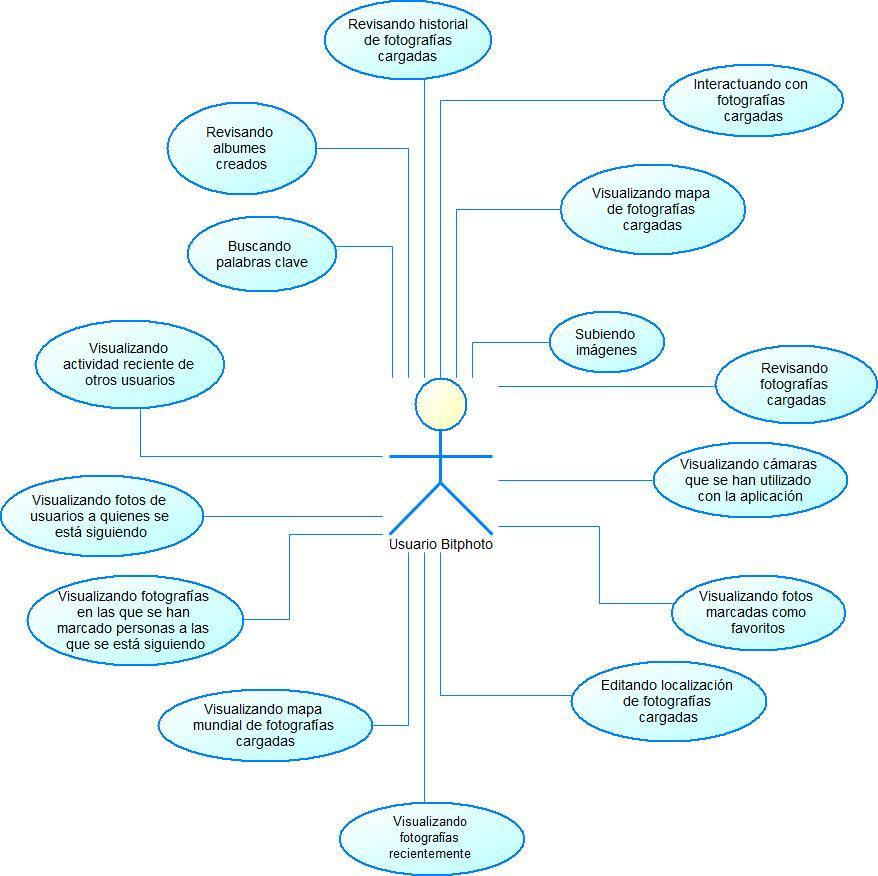
\includegraphics[width=16.5cm]{DiagramaDeCasosDeUso.jpg}
}

\newpage
\tabla{Caso de Uso CU01: Revisando historial de fotografías cargadas.}{
	\begin{tabular}[c]{|p{2.7cm}|p{13.3cm}|}
		\hline
		\textbf{ID}  & CU01\\ \hline
		\textbf{Nombre} & Revisando historial de fotografías cargadas\\ \hline
		\textbf{Resumen} & El usuario puede ver sus fotografías cargadas al sistema, agrupadas por la fecha en que fueron tomadas o subidas a la aplicación.\\ \hline
		\textbf{Actores} & Usuario\\ \hline
		\textbf{Precondiciones} & El usuario inicia sesión en el sistema ingresando cuenta y contraseña válidas.\\ \hline
		\textbf{Descripción} & El usuario, luego de iniciar sesión y encontrarse en la página principal del sistema, selecciona la opción “Camera Roll”. Luego de encontrarse en la vista “Camera Roll”, se muestran todas las fotografías que ha subido el usuario a la aplicación agrupadas la fecha en que fueron subidas a la plataforma, luego selecciona la opción “fecha de toma”, luego se muestra la vista “Camera Roll” con las fotografías del usuario agrupadas por la fecha en que fueron tomadas por el usuario. (EX01: El usuario no ha subido fotografías a la aplicación). Luego, el usuario selecciona cualquiera de las fotografías que se muestran para revisar toda la información asociada, como los comentarios, cantidad de favoritos, entre otras.\\ \hline
		\textbf{Postcondiciones} & El usuario se encuentra en la vista “Camera Roll” visualizando las fotografias propias subidas a la aplicación, permitiéndole escoger cualquiera de ellas para revisar su información.\\ \hline
		\textbf{Requisitos de Usabilidad} & El sistema indica al usuario que se encuentra en la vista “Camera Roll” mediante un título o un encabezado en la página.\\ \hline
		\textbf{Excepciones} & \textbf{Ex01: El usuario no ha subido fotografías a la aplicación.}
		
Puede suceder que el usuario aún no suba fotografías a la aplicación, por lo tanto, se le informará por pantalla que no ha subido fotografías a la aplicación.
\\ \hline
	\end{tabular}
}

\newpage
\tabla{Caso de Uso CU02: Revisando fotografías cargadas.}{
	\begin{tabular}[c]{|p{2.7cm}|p{13.3cm}|}
		\hline
		\textbf{ID}  & CU02\\ \hline
		\textbf{Nombre} & Revisando fotografías cargadas\\ \hline
		\textbf{Resumen} & El usuario puede ver las fotografías que ha subido a la aplicación ordenadas por fechas en que fueron subidas o fecha en que fueron tomadas.\\ \hline
		\textbf{Actores} & Usuario\\ \hline
		\textbf{Precondiciones} & El usuario inicia sesión en el sistema ingresando cuenta y contraseña válidas.\\ \hline
		\textbf{Descripción} & El usuario, luego de iniciar sesión y encontrarse en la página principal del sistema, selecciona la opción “Photostream”. Luego de encontrarse en la vista “Photostream”, se muestran las fotografías del usuario ordenadas por la fecha en que fueron subidas a la aplicación. (EX01: No existen fotografías del usuarios). A continuación el usuario selecciona la opción “fecha de toma”, ahora en la vista “photostream” se muestran las fotos del usuario ordenadas por la fecha en fueron tomas.(EX01: No existen fotografías del usuarios). Luego, el usuario selecciona cualquiera de las fotografías que se muestran para revisar toda la información asociada, como los comentarios, cantidad de favoritos, entre otras.\\ \hline
		\textbf{Postcondiciones} & El usuario se encuentra en la vista “photostream” visualizando todas las fotografías de otros usuarios, permitiéndole escoger cualquiera de ellas para revisar su información.\\ \hline
		\textbf{Requisitos de Usabilidad} & El sistema indica al usuario que se encuentra en la vista “Photostream” mediante un título o un encabezado en la página.\\ \hline
		\textbf{Excepciones} & \textbf{Ex01: No existen fotografías del usuario.}

Puede suceder que el usuario aún no suba fotografías a la aplicación, por lo tanto, se le informará por pantalla que no ha subido fotografías a la aplicación. 
\\ \hline
	\end{tabular}
}

\newpage
\tabla{Caso de Uso CU03: Revisando álbumes creados.}{
	\begin{tabular}[c]{|p{2.7cm}|p{13.3cm}|}
		\hline
		\textbf{ID}  & CU03\\ \hline
		\textbf{Nombre} & Revisando álbumes creados\\ \hline
		\textbf{Resumen} & El usuario puede ver los álbumes que ha creado en el sistema, además puede ver qué fotografías se encuentran en cada álbum.\\ \hline
		\textbf{Actores} & Usuario\\ \hline
		\textbf{Precondiciones} & El usuario inicia sesión en el sistema ingresando cuenta y contraseña válidas.\\ \hline
		\textbf{Descripción} & El usuario, luego de iniciar sesión y encontrarse en la página principal del sistema, selecciona la opción “Álbumes”. Luego de encontrarse en la vista “Álbumes”, se muestran los álbumes que el usuario a creado.(EX01: El usuario no ha creado ningún álbum). El usuario selecciona un álbum, luego se muestra en la vista “Álbumes” las fotografías contenidas en este. Luego, el usuario selecciona cualquiera de las fotografías que se muestran para revisar toda la información asociada, como los comentarios, cantidad de favoritos, entre otras.\\ \hline
		\textbf{Postcondiciones} & El usuario se encuentra en la vista “Álbumes” visualizando los álbumes creados, permitiéndole escoger un álbum y revisar que fotográficas contiene, además de permitirle seleccionar cualquier fotografía para poder revisar su información.\\ \hline
		\textbf{Requisitos de Usabilidad} & El sistema indica al usuario que se encuentra en la vista “Álbumes” mediante un título o un encabezado en la página.\\ \hline
		\textbf{Excepciones} & \textbf{Ex01: El usuario no ha creado ningún álbum.}

Existe la posibilidad de que el usuario no haya creado ningún álbum, en este caso, se le informa que no existen álbumes.
\\ \hline
	\end{tabular}
}

\newpage
\tabla{Caso de Uso CU04: Visualizando mapa de fotografías cargadas.}{
	\begin{tabular}[c]{|p{2.7cm}|p{13.3cm}|}
		\hline
		\textbf{ID}  & CU04\\ \hline
		\textbf{Nombre} & Visualizando mapa de fotografías cargadas\\ \hline
		\textbf{Resumen} & El usuario podrá visualizar un mapa en el que ha localizado las fotografías que ha cargado a la aplicación.\\ \hline
		\textbf{Actores} & Usuario\\ \hline
		\textbf{Precondiciones} & El usuario inicia sesión en el sistema ingresando cuenta y contraseña válidas.\\ \hline
		\textbf{Descripción} & El usuario, luego de iniciar sesión y encontrarse en la página principal del sistema, selecciona la opción “Mapa”. Luego de encontrarse en la vista “Mapa”, se muestra un mapa donde el usuario ha localizado las fotografías que ha cargado a la aplicación, mostrándose la ubicación con un punto (EX01: El usuario no ha localizado ninguna fotografía.). Posteriormente el usuario selecciona cualquiera de las fotografías encontradas en el mapa para observar toda la información que esté asociada a ésta (comentarios, personas marcadas, entre otros).  \\ \hline
		\textbf{Postcondiciones} & El usuario se encuentra en la vista “Mapa” visualizando las fotografías localizadas. \\ \hline
		\textbf{Requisitos de Usabilidad} & El sistema indica al usuario que se encuentra en la vista “Mapa” mediante un título o un encabezado en la página.\\ \hline
		\textbf{Excepciones} & \textbf{Ex01: El usuario no ha localizado ninguna fotografía.}

Si el usuario no ha asignado ninguna ubicación a las fotografías que ha cargado a la página, el mapa se mostrará de igual manera informándole a través de un mensaje que no ha localizado ninguna fotografía.
\\ \hline
	\end{tabular}
}

\newpage
\tabla{Caso de Uso CU05: Editanto localización de fotografías cargadas.}{
	\begin{tabular}[c]{|p{2.7cm}|p{13.3cm}|}
		\hline
		\textbf{ID}  & CU05\\ \hline
		\textbf{Nombre} & Editanto localización de fotografías cargadas\\ \hline
		\textbf{Resumen} & El usuario puede editar la localización de las fotografías que ha cargado en la aplicación.\\ \hline
		\textbf{Actores} & Usuario\\ \hline
		\textbf{Precondiciones} & El usuario inicia sesión en el sistema ingresando cuenta y contraseña válidas.\\ \hline
		\textbf{Descripción} & El usuario, luego de iniciar sesión y encontrarse en la página principal del sistema, selecciona la opción “Editar Fotografía”. Luego de encontrarse en la vista “Editar Fotografía”, selecciona la opción “Editar Ubicación”, correspondiente a la opción para cambiar la localización de la fotografía en el mapa. Posteriormente el usuario ingresa el nombre del país en el que desea ubicar la fotografía (EX01: El país ingresado no es válido) y finaliza la edición. Por último, se mostrará en el mapa el país al que ha sido asociada la fotografía y éste aparecerá en la información al momento de revisar la misma.\\ \hline
		\textbf{Postcondiciones} & El usuario se encuentra en la vista “Editar Fotografía” donde aparecen todas las opciones de edición dentro de las que se muestra “Editar Ubicación”.\\ \hline
		\textbf{Requisitos de Usabilidad} & El sistema indica al usuario que se encuentra en la vista “Editar Fotografía” mediante un título o un encabezado en la página.\\ \hline
		\textbf{Excepciones} & \textbf{Ex01: El país ingresado no es válido.}
		
Puede suceder que el usuario, al momento de ingresar el país en el que desea ubicar la fotografía, ingrese el nombre mal escrito, o ingrese números u otros caracteres no válidos, en este caso se le muestra un mensaje de alerta informándole del error y solicitando que ingrese el nombre nuevamente.
\\ \hline
	\end{tabular}
}

\newpage
\tabla{Caso de Uso CU06: Visualizando fotografías marcadas como favoritos.}{
	\begin{tabular}[c]{|p{2.7cm}|p{13.3cm}|}
		\hline
		\textbf{ID}  & CU06\\ \hline
		\textbf{Nombre} & Visualizando fotografías marcadas como favoritos\\ \hline
		\textbf{Resumen} & El usuario puede ver las fotografías en las que ha marcado la opción “favoritos”.\\ \hline
		\textbf{Actores} & Usuario\\ \hline
		\textbf{Precondiciones} & El usuario inicia sesión en el sistema ingresando cuenta y contraseña válidas.\\ \hline
		\textbf{Descripción} & El usuario, luego de iniciar sesión puede revisar la información asociada de cualquier fotografía en las vistas correspondientes (vista “Explorar”, en el perfil de un amigo, mapa del mundo, entre otras) y marcar la opción “Favorito” si es que lo desea. Luego, todas las fotografías en las que haya marcado esta opción, se encontrarán en la vista “Favoritos”, donde el usuario puede revisar la información asociada en cualquier momento. \\ \hline
		\textbf{Postcondiciones} & El usuario se encuentra en la vista “Favoritos” visualizando todas las fotografías en las que se ha marcado la opción “Favorito”.\\ \hline
		\textbf{Requisitos de Usabilidad} & El sistema indica al usuario que se encuentra en la vista “Favoritos” mediante un título o un encabezado en la página.\\ \hline
		\textbf{Excepciones} & \\ \hline
	\end{tabular}
}

\newpage
\tabla{Caso de Uso CU07: Visualizando actividad reciente de otros usuarios.}{
	\begin{tabular}[c]{|p{2.7cm}|p{13.3cm}|}
		\hline
		\textbf{ID}  & CU07\\ \hline
		\textbf{Nombre} & Visualizando actividad reciente de otros usuarios\\ \hline
		\textbf{Resumen} & El usuario puede ver la actividad reciente de otros usuarios relacionadas con él mismo (ya sea en las fotografías del usuario, respuestas a los comentarios del usuario, entre otros).\\ \hline
		\textbf{Actores} & Usuario\\ \hline
		\textbf{Precondiciones} & El usuario inicia sesión en el sistema ingresando cuenta y contraseña válidas.\\ \hline
		\textbf{Descripción} & El usuario, luego de iniciar sesión y encontrarse en la página principal del sistema, selecciona la opción “Actividad Reciente”. Luego de encontrarse en la vista “Actividad Reciente”, se muestra toda actividad de otras personas que esté relacionada con el usuario, por ejemplo, respuesta a sus comentarios, actividad en las fotografías que ha cargado al sistema, nuevos seguidores, entre otras (EX01: No existe actividad reciente de otros usuarios).  \\ \hline
		\textbf{Postcondiciones} & El usuario se encuentra en la vista “Actividad Reciente” visualizando toda la actividad de otros usuarios. \\ \hline
		\textbf{Requisitos de Usabilidad} & El sistema indica al usuario que se encuentra en la vista “Actividad Reciente” mediante un título o un encabezado en la página.\\ \hline
		\textbf{Excepciones} & \textbf{Ex01: No existen actividad reciente de otros usuarios.}
		
Puede suceder que no existan actividades de otras personas relacionadas con el usuario, por lo tanto, se le informará por pantalla que no ha habido interacciones.
\\ \hline
	\end{tabular}
}

\newpage
\tabla{Caso de Uso CU08: Viendo fotografías de usuarios a quienes se sigue.}{
	\begin{tabular}[c]{|p{2.7cm}|p{13.3cm}|}
		\hline
		\textbf{ID}  & CU08\\ \hline
		\textbf{Nombre} & Visualizando fotografías de usuarios a quienes se está siguiendo\\ \hline
		\textbf{Resumen} & El usuario puede ver las fotografías de las personas que está siguiendo escogiendo entre ver 1 o 5 fotografías por persona.\\ \hline
		\textbf{Actores} & Usuario\\ \hline
		\textbf{Precondiciones} & El usuario inicia sesión en el sistema ingresando cuenta y contraseña válidas.\\ \hline
		\textbf{Descripción} & El usuario, luego de iniciar sesión y encontrarse en la página principal del sistema, selecciona la opción “Fotos de”. Luego de encontrarse en la vista “Fotos de”, se muestran las fotografías de las personas a las que está siguiendo (EX01: No hay fotografías de otros usuarios). Dependiendo del filtro de la cantidad de fotografías que el usuario escoja, verá 1 o 5 fotografías por cada persona que está siguiendo (EX02: Uno o más usuarios tiene menos de 5 fotografías). Luego, el usuario selecciona cualquier fotografía que se muestre para ver toda la información asociada, como comentarios, cantidad de favoritos, entre otras.\\ \hline
		\textbf{Postcondiciones} & El usuario se encuentra en la vista “Fotos de” viendo todas las fotografías de otros usuarios, permitiéndole escoger cualquiera para ver la información.\\ \hline
		\textbf{Requisitos de Usabilidad} & El sistema indica al usuario que se encuentra en la vista “Fotos de” mediante un título o un encabezado en la página.\\ \hline
		\textbf{Excepciones} & \textbf{Ex01: No hay fotografías de otros usuarios.}
		
Es posible que el usuario esté siguiendo solamente a personas que no hayan subido ninguna fotografía, en este caso, se le informa que las personas que sigue no han subido fotografías y se le recomienda seguir a otros usuarios.

\textbf{Ex02: Uno o más usuarios tiene menos de 5 fotografías.}

En caso que el usuario desee ver 5 fotografías por persona y haya una o más personas que no tengan esa cantidad de fotografías cargadas, de igual forma se hace el filtro correspondiente y se muestran las fotografías que tengan (por ejemplo, si un usuario solo tiene 3 fotografías, se hace el filtro por 5 y solo se muestran las que se han cargado).  
\\ \hline
	\end{tabular}
}

\newpage
\tabla{Caso de Uso CU09: Visualizando fotografías en las que se han marcado personas a las que se está siguiendo.}{
	\begin{tabular}[c]{|p{2.7cm}|p{13.3cm}|}
		\hline
		\textbf{ID}  & CU09\\ \hline
		\textbf{Nombre} & Visualizando fotografías en las que se han marcado personas a las que se está siguiendo\\ \hline
		\textbf{Resumen} & El usuario puede ver las fotografías de cualquier persona, en las que se ha marcado a otros usuarios que está siguiendo.\\ \hline
		\textbf{Actores} & Usuario\\ \hline
		\textbf{Precondiciones} & El usuario inicia sesión en el sistema ingresando cuenta y contraseña válidas.\\ \hline
		\textbf{Descripción} & El usuario, luego de iniciar sesión y encontrarse en la página principal del sistema, selecciona la opción “Fotos con”. Luego de encontrarse en la vista “Fotos con”, se muestran las fotografías en las se ha marcado a personas a las que está siguiendo (EX01: Ninguna persona a la que sigue el usuario se ha marcado en alguna fotografía). Las fotografías en la que se han marcado las personas a las que el usuario sigue pueden ser de cualquier persona, incluso personas que no está siguiendo. Luego, el usuario selecciona cualquiera de las fotografías que se muestran para revisar toda la información asociada, como los comentarios, cantidad de favoritos, entre otras.\\ \hline
		\textbf{Postcondiciones} & El usuario se encuentra en la vista “Fotos con” visualizando todas las fotografías en las que se ha marcado a otros usuarios, permitiéndole escoger cualquiera de ellas para revisar la información.\\ \hline
		\textbf{Requisitos de Usabilidad} & El sistema indica al usuario que se encuentra en la vista “Fotos con” mediante un título o un encabezado en la página.\\ \hline
		\textbf{Excepciones} & \textbf{Ex01: Ninguna persona a la que sigue el usuario se ha marcado en alguna fotografía.}
		
Existe la posibilidad que no se marque en ninguna fotografía a ninguna de las personas que el usuario está siguiendo, en este caso, se le informa que no existen dichas fotografías.
\\ \hline
	\end{tabular}
}

\newpage
\tabla{Caso de Uso CU10: Visualizando fotografías recientemente cargadas a la aplicación.}{
	\begin{tabular}[c]{|p{2.7cm}|p{13.3cm}|}
		\hline
		\textbf{ID}  & CU10\\ \hline
		\textbf{Nombre} & Visualizando fotografías recientemente cargadas a la aplicación\\ \hline
		\textbf{Resumen} & El usuario podrá ver una fotografía de las que se han subido recientemente a la aplicación por todos los usuarios de ésta.\\ \hline
		\textbf{Actores} & Usuario\\ \hline
		\textbf{Precondiciones} & El usuario inicia sesión en el sistema ingresando cuenta y contraseña válidas.\\ \hline
		\textbf{Descripción} & El usuario selecciona la opción fotos recientes, donde el sistema muestra en la vista correspondiente las fotografías filtradas, el usuario selecciona una de éstas fotografías, por lo que el sistema responde mostrando solo ésta, junto con sus comentarios, descripción, fecha de carga y cantidad de favoritos según corresponda.\\ \hline
		\textbf{Postcondiciones} & El sistema muestra una fotografía en detalle.\\ \hline
		\textbf{Requisitos de Usabilidad} & El sistema indica al usuario que se encuentra en la vista “Fotos Recientes” mediante un título o un encabezado en la página.\\ \hline
		\textbf{Excepciones} & \\ \hline
	\end{tabular}
}

\newpage
\tabla{Caso de Uso CU11: Visualizando mapa mundial de fotografías cargadas.}{
	\begin{tabular}[c]{|p{2.7cm}|p{13.3cm}|}
		\hline
		\textbf{ID}  & CU11\\ \hline
		\textbf{Nombre} & Visualizando mapa mundial de fotografías cargadas\\ \hline
		\textbf{Resumen} & El usuario puede ver fotografías que se encuentran en un país a seleccionar en el mapa.\\ \hline
		\textbf{Actores} & Usuario\\ \hline
		\textbf{Precondiciones} & El usuario inicia sesión en el sistema ingresando cuenta y contraseña válidas.\\ \hline
		\textbf{Descripción} & El usuario debe seleccionar la opción mapa mundial, por lo que el sistema responde cargando en una vista el mapa correspondiente, donde el usuario procede a seleccionar un país en el cual desea buscar fotografías, por lo que el sistema carga las imágenes ubicadas en el país correspondiente (Ex 1: No existen fotografías asociadas con la ubicación).\\ \hline
		\textbf{Postcondiciones} & El sistema carga las fotografías asociadas a la ubicación seleccionada.\\ \hline
		\textbf{Requisitos de Usabilidad} & El sistema indica al usuario que se encuentra en la vista “Mapa del Mundo” mediante un título o un encabezado en la página.\\ \hline
		\textbf{Excepciones} & \textbf{Ex01: No existen fotografías asociadas a la ubicación.}
		
El sistema avisa al usuario que la ubicación seleccionada no tiene fotografías asociadas.
\\ \hline
	\end{tabular}
}

\newpage
\tabla{Caso de Uso CU12: Visualizando cámaras que se han utilizado con la aplicación.}{
	\begin{tabular}[c]{|p{2.7cm}|p{13.3cm}|}
		\hline
		\textbf{ID}  & CU12\\ \hline
		\textbf{Nombre} & Visualizando cámaras que se han utilizado con la aplicación\\ \hline
		\textbf{Resumen} & El usuario puede ver las cámaras y sus características correspondientemente. \\ \hline
		\textbf{Actores} & Usuario\\ \hline
		\textbf{Precondiciones} & El usuario inicia sesión en el sistema ingresando cuenta y contraseña válidas.\\ \hline
		\textbf{Descripción} & El usuario selecciona la opción cámaras, por lo que el sistema carga éstas y muestra un ranking de las cámaras más utilizadas en la aplicación, luego el usuario selecciona una de las cámaras, así el sistema muestra las características de la cámara seleccionada.\\ \hline
		\textbf{Postcondiciones} & El sistema carga en una vista las características de la cámara específicamente seleccionada.\\ \hline
		\textbf{Requisitos de Usabilidad} & El sistema indica al usuario que se encuentra en la vista “Buscador de Cámaras” mediante un título o un encabezado en la página.\\ \hline
		\textbf{Excepciones} & \\ \hline
	\end{tabular}
}

\newpage
\tabla{Caso de Uso CU13: Buscando palabra clave.}{
	\begin{tabular}[c]{|p{2.7cm}|p{13.3cm}|}
		\hline
		\textbf{ID}  & CU13\\ \hline
		\textbf{Nombre} & Buscando palabra clave\\ \hline
		\textbf{Resumen} & El usuario puede buscar una palabra clave en la sección del buscador (ya sea para encontrar fotografías con la palabra en tags, en el nombre, descripción o comentarios o otros usuarios que contengan la palabra en su nombre de usuario).\\ \hline
		\textbf{Actores} & Usuario\\ \hline
		\textbf{Precondiciones} & El usuario inicia sesión en el sistema ingresando cuenta y contraseña válidas.\\ \hline
		\textbf{Descripción} & El usuario, luego de iniciar sesión y encontrarse en la página principal del sistema, escribe una o más palabras en el buscador y luego selecciona buscar, al encontrarse en la vista “Buscador” este muestra todas las coincidencias con la o las palabras claves insertadas por el usuario(EX01: no existen coincidencias con la búsqueda realizada).  \\ \hline
		\textbf{Postcondiciones} & El usuario se encuentra en la vista “Busqueda”, visualizando las coincidencias encontradas por el buscador.\\ \hline
		\textbf{Requisitos de Usabilidad} & El sistema indica al usuario que se encuentra en la vista “Busqueda” mediante un título o un encabezado en la página.\\ \hline
		\textbf{Excepciones} & \textbf{Ex01: No existen coincidencias con la búsqueda realizada.}
		
Puede suceder que no existan coincidencias de búsqueda con la o palabras claves ingresadas, en ese caso el sistema informara que no se pudo encontrar nada con la información recibida.
\\ \hline
	\end{tabular}
}

\newpage
\tabla{Caso de Uso CU14: Subiendo imágenes.}{
	\begin{tabular}[c]{|p{2.7cm}|p{13.3cm}|}
		\hline
		\textbf{ID}  & CU14\\ \hline
		\textbf{Nombre} & Subiendo imágenes\\ \hline
		\textbf{Resumen} & El usuario sube imagen y edita sus campos(Agregar descripción, tags, personas, etc).\\ \hline
		\textbf{Actores} & Usuario\\ \hline
		\textbf{Precondiciones} & El usuario inicia sesión en el sistema ingresando cuenta y contraseña válidas.\\ \hline
		\textbf{Descripción} & El usuario, luego de iniciar sesión y encontrarse en la página principal del sistema, selecciona la opción “Subir foto”. Luego de encontrarse en la vista “Subir foto”, se muestran las opciones que puede llenar, para la información de la fotografía.(EX01: No existe una fotografía para subir o no es del formato valido). El usuario rellena los distintos campos de la información de la fotografía y selecciona “Subir foto”.\\ \hline
		\textbf{Postcondiciones} & El usuario se puede visualizar la fotografía recientemente subida al sistema.\\ \hline
		\textbf{Requisitos de Usabilidad} & El sistema indica al usuario que se encuentra en la vista “Subir foto” mediante un título o un encabezado en la página.\\ \hline
		\textbf{Excepciones} & \textbf{Ex01: No existe una fotografía para subir.}
		
El usuario no ha seleccionado una fotografía para subir al sistema, el sistema le indica por pantalla que no ha seleccionado una fotografía o que esta no es válida para subir, ya sea por el formato u otro problema, para esto el usuario debe seleccionar una fotografía valida para editar y subir al sistema.
\\ \hline
	\end{tabular}
}

\newpage
\tabla{Caso de Uso CU15: Interactuando con fotografías cargadas.}{
	\begin{tabular}[c]{|p{2.7cm}|p{13.3cm}|}
		\hline
		\textbf{ID}  & CU15\\ \hline
		\textbf{Nombre} & Interactuando con fotografías cargadas\\ \hline
		\textbf{Resumen} & El usuario puede ver la información de alguna  fotografía cargada y agregar información a esta fotografía (ya sea agregar comentario, marcar como favorito, agregar personas, etc).\\ \hline
		\textbf{Actores} & Usuario\\ \hline
		\textbf{Precondiciones} & El usuario inicia sesión en el sistema ingresando cuenta y contraseña válidas.\\ \hline
		\textbf{Descripción} & El usuario, luego de iniciar sesión y encontrarse en la página principal del sistema, selecciona la fotografía que quiere visualizar, el usuario interactúa con la fotografía (Agregando comentario, marcando como favorito, agregando personar, agregando tags), luego el sistema guarda los cambios y de la fotografía y se encuentra nuevamente visualizando la fotografía con la información agregada realizados.\\ \hline
		\textbf{Postcondiciones} & El usuario se encuentra en la vista visualizando la foto con la que realizo una interacción y puede observar la interaccione realizada, que cambio alguna información de la fotografía.\\ \hline
		\textbf{Requisitos de Usabilidad} & El sistema indica al usuario el cambio que se realiza en la fotografía.\\ \hline
		\textbf{Excepciones} & \\ \hline
	\end{tabular}
}


%-------------------------------------------------------------------------------------
\capitulo{DIAGRAMAS DE SECUENCIA.}

A continuación, se muestran los diagramas de secuencia para plasmar el modelo de comportamiento de los casos de uso que se desearon implementar.

%\figura{Implementación login.}{
%	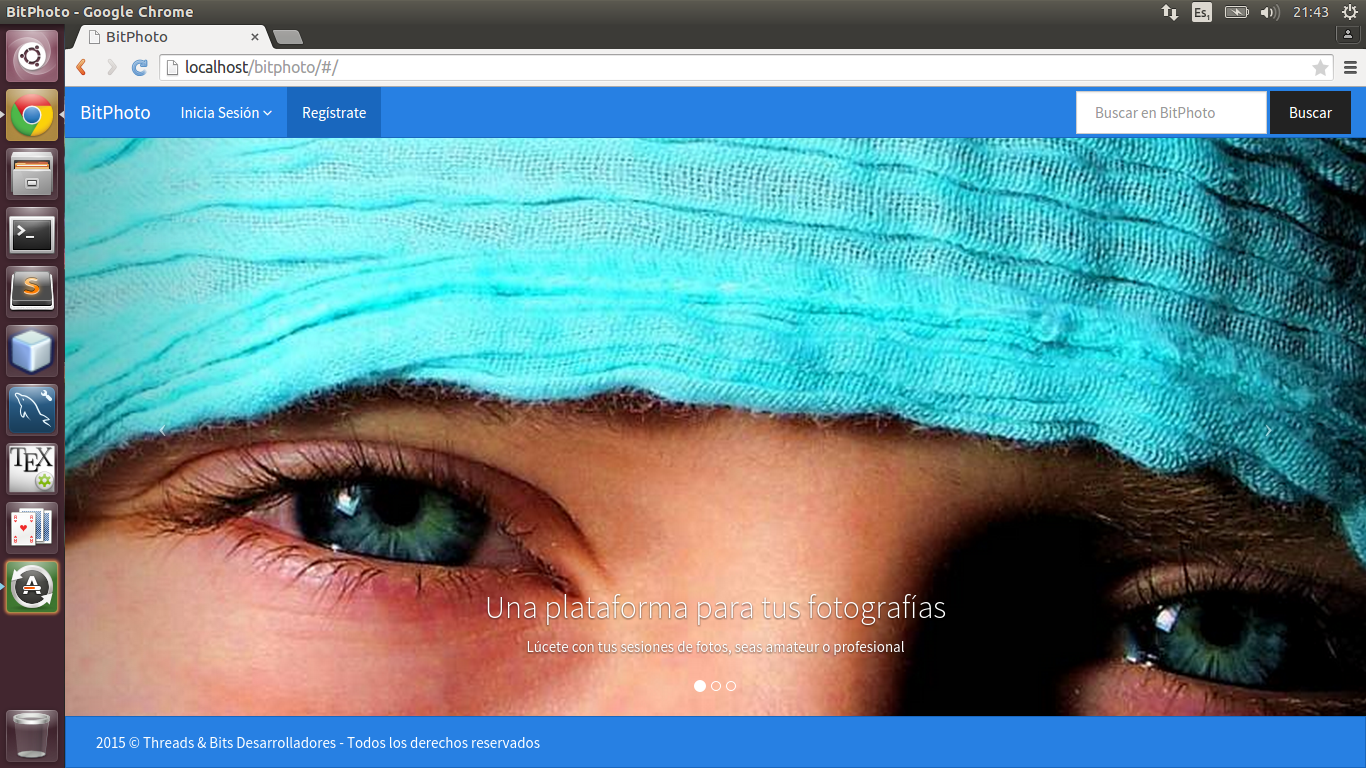
\includegraphics[width=16.5cm]{login1.png}
%}

%\figura{Implementación login.}{
%	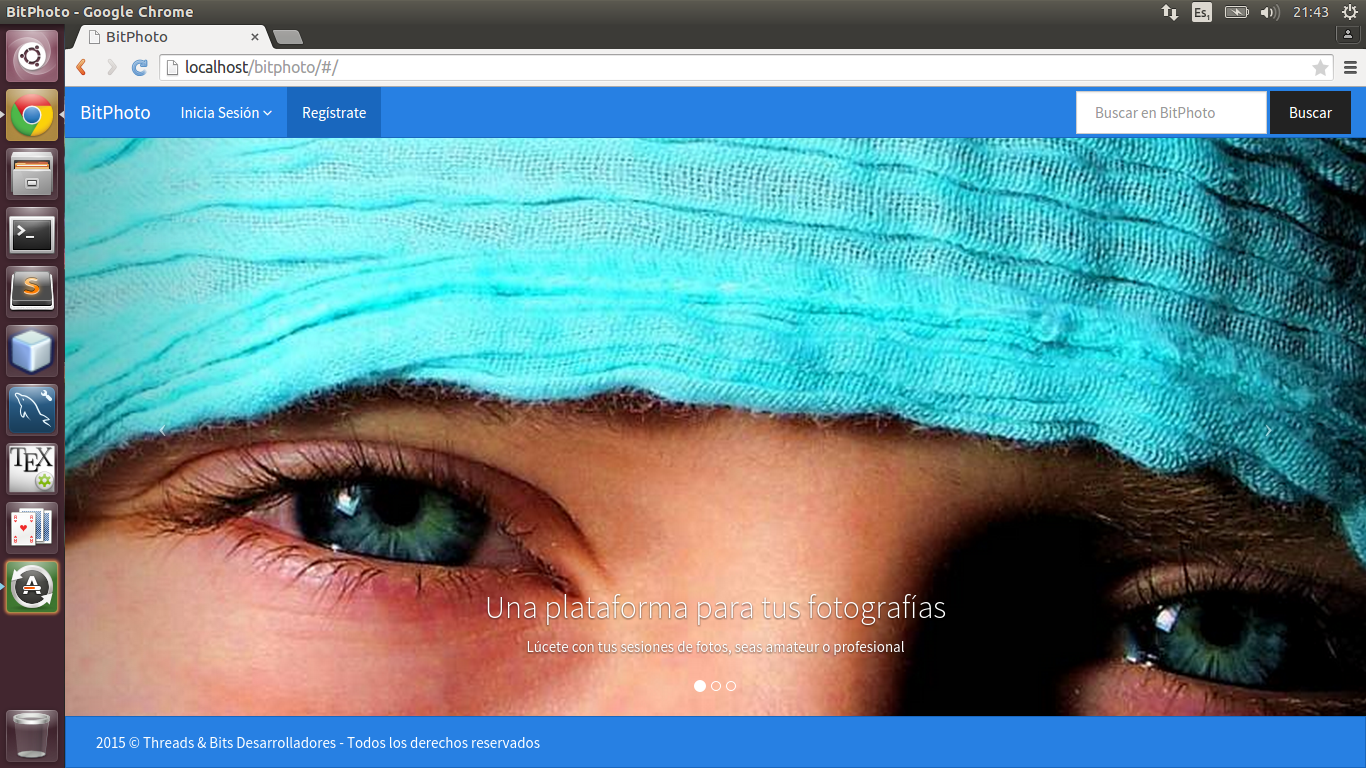
\includegraphics[width=16.5cm]{login1.png}
%}

%-------------------------------------------------------------------------------------
\capitulo{DETALLE DE CASOS DE USO IMPLEMENTADOS.}

Si bien se planificó dentro de los Casos de Uso la implementación de la vista de fotografías y álbumes, se decidió comenzar en la implementación por una precondición necesaria para ambos Casos de Uso: El Inicio de Sesión y el Registro.

Tomando como base el Prototipo mostrado en entregas anteriores, se cambió el sistema de navegación por Rutas de \textsl{AngularJS}:

\figura{Implementación, pantalla principal.}{
	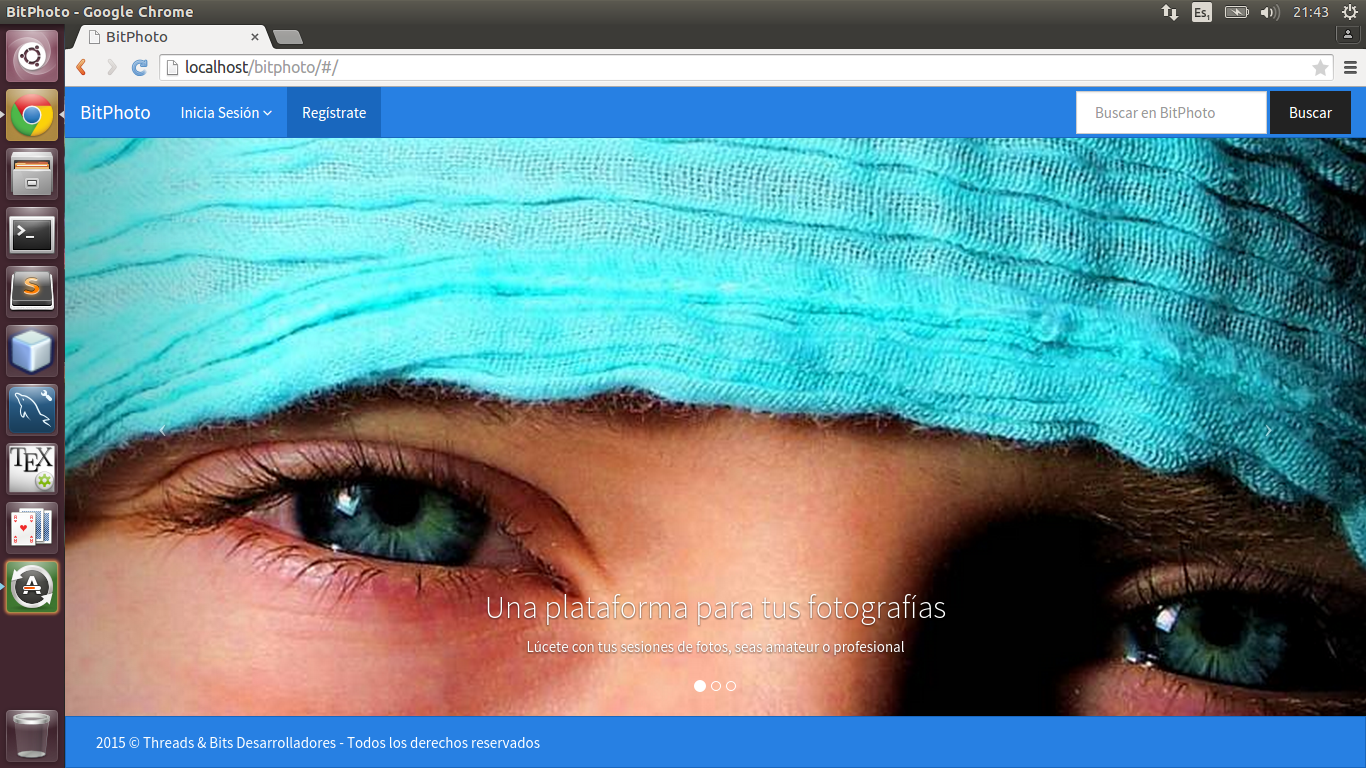
\includegraphics[width=16cm]{login1.png}
}

Si bien no es un cambio notorio en la vista como tal, el usar el módulo de navegación nativo de \textsl{AngularJS} permite cargar controladores en cualquier vista de la aplicación web.

Luego se procedió a implementar la validación de formularios potenciada por \textsl{AngularJS}, la cual permite verificar que los datos tengan contenido admisible por el campo en cuestión (por ejemplo, que una dirección de correo electrónico tenga una arroba).

\figura{Implementación registro.}{
	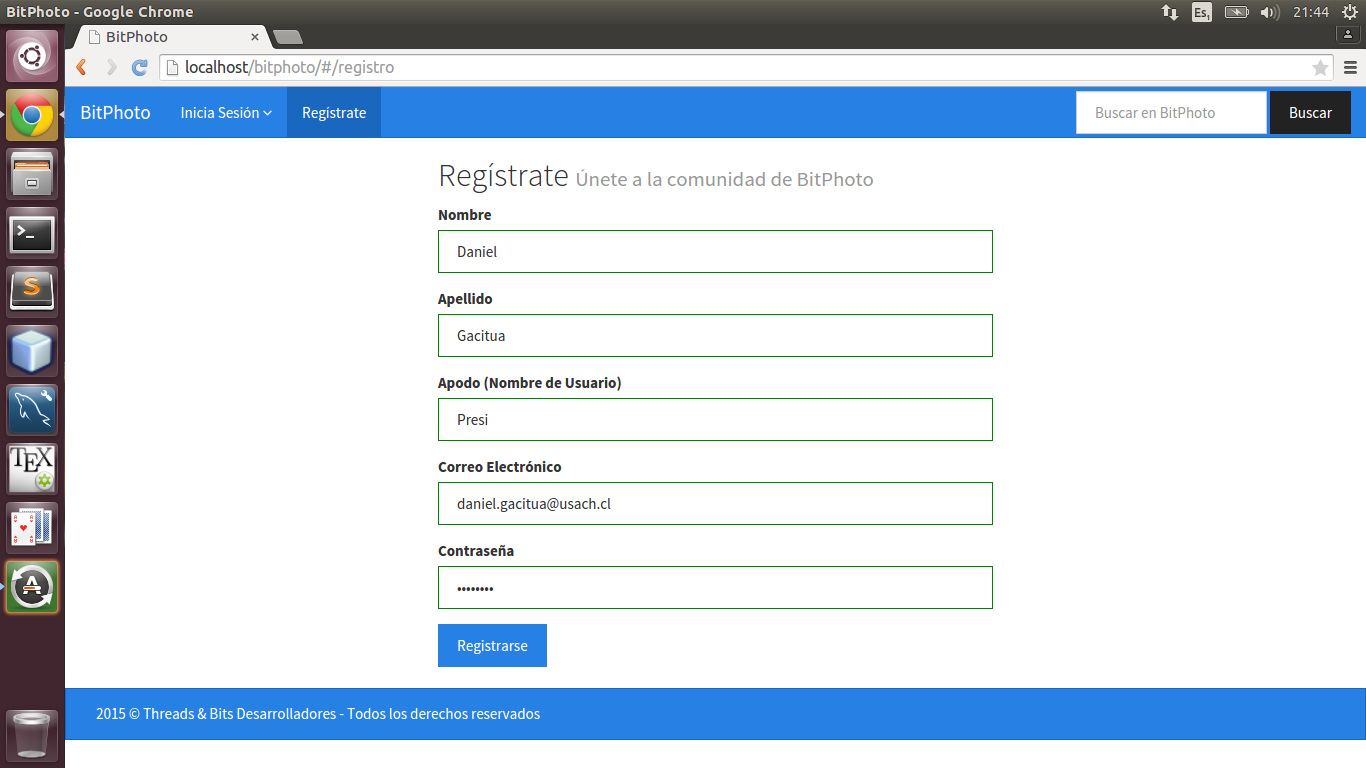
\includegraphics[width=16cm]{login2.png}
}

Con estos elementos terminados, se construyó el código de autenticación en \textsl{AngularJS} para el Inicio de Sesión y el Registro. Como aún no se ha podido realizar la integración de servicios \textsl{REST} con \textsl{JavaEE}, se implementó un servicio \textsl{REST} falso (basado en \textsl{LocalStorage}) para guardar los datos de registro.

\figura{Implementación login.}{
	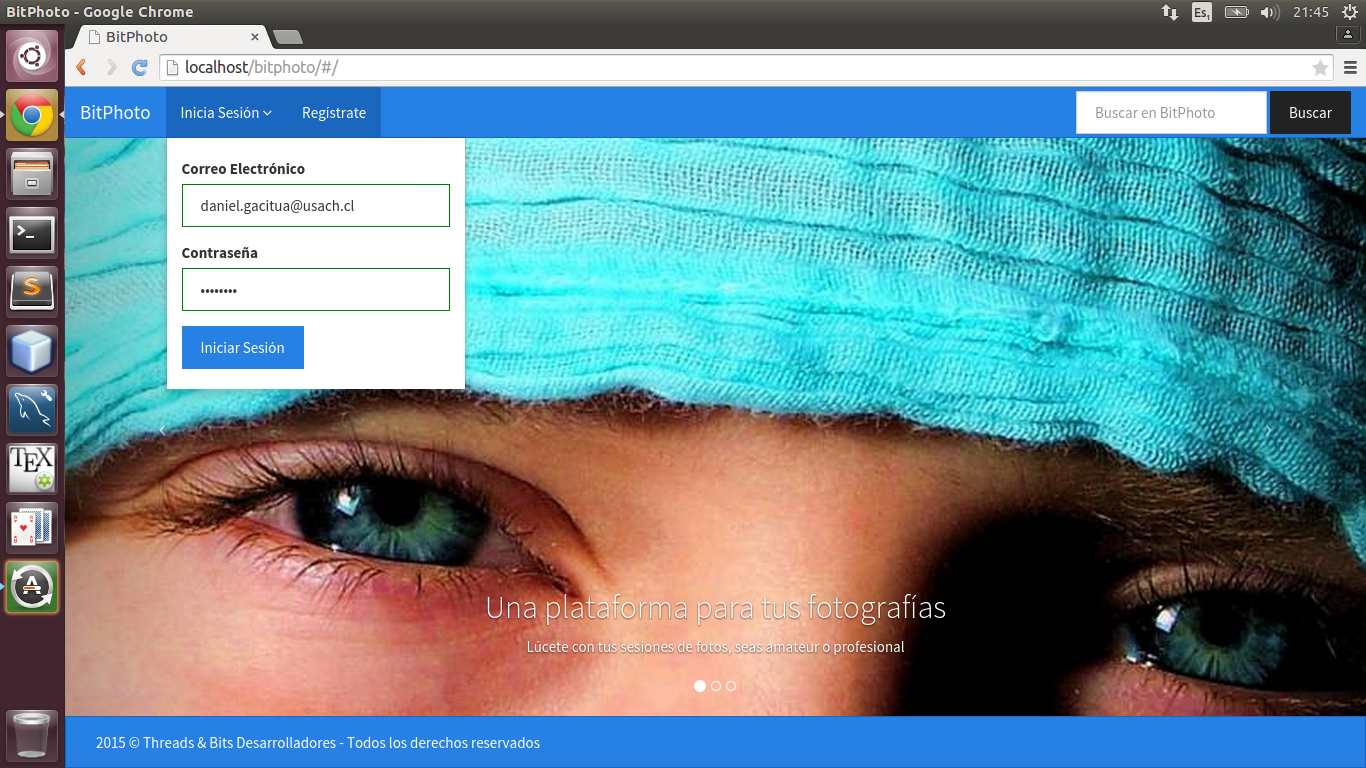
\includegraphics[width=16cm]{login3.png}
}

El sistema de autenticación actual tiene la facultad de crear \textsl{cookies} de navegador que permiten la persistencia de la sesión, y obtener datos adicionales y personalizados de cada usuario.

\figura{Implementación, subir fotografía.}{
	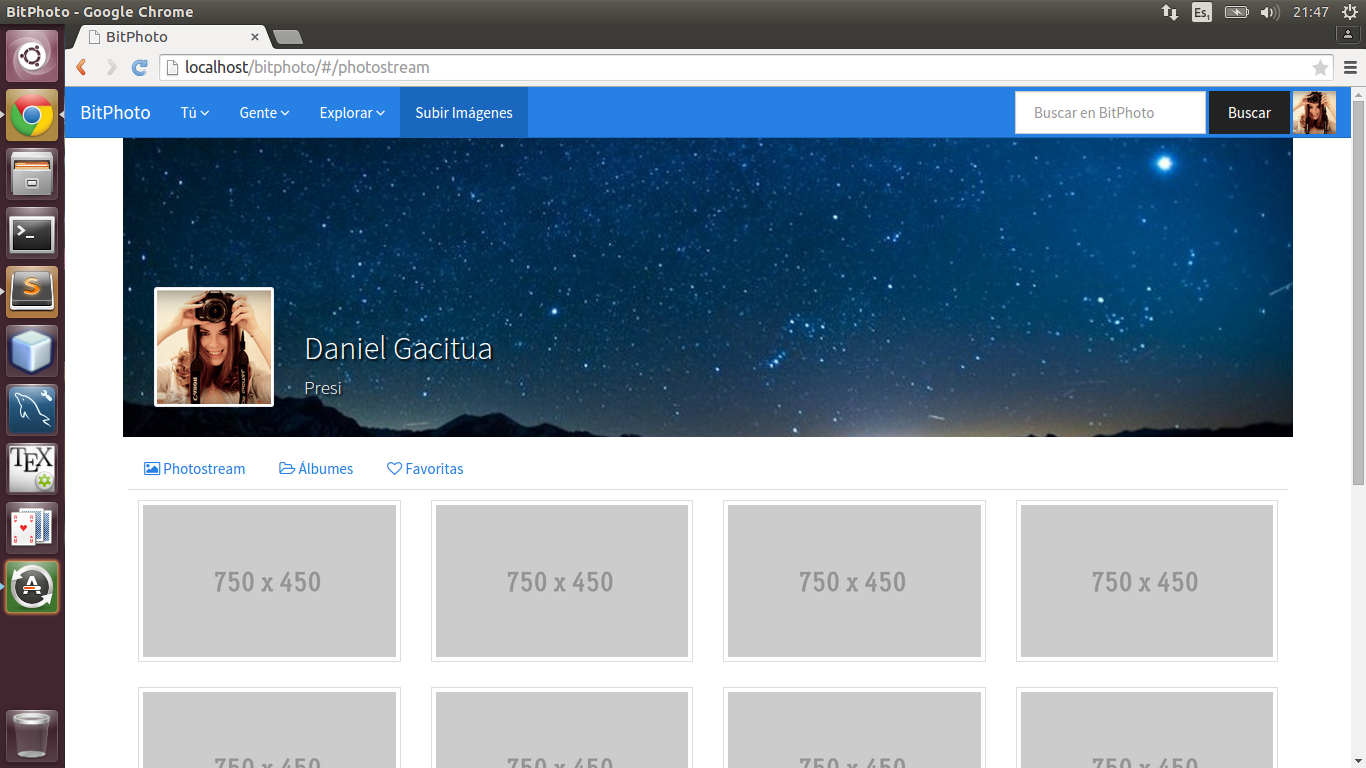
\includegraphics[width=16cm]{login4.png}
}

Las imágenes y otros elementos aún permanecen estáticos, y serán implementados en entregas posteriores, basados en la implementación recién mencionada.


%-------------------------------------------------------------------------------------
\capitulo{GESTIÓN DEL PROYECTO.}

\seccion{ORGANIZACIÓN DE REPOSITORIOS GIT.}
    
Para optimizar la creación de código, favorecer la correcta colaboración entre los integrantes y tener un versionamiento ordenado del código, se decide emplear a git como sistema de control de versiones, y usar GitHub como servidor remoto de git.\\

Cada miembro del grupo utiliza una cuenta de GitHub:

\begin{itemize}
	\item \textbf{Gerson Aguirre}: \textsl{https://github.com/GersonAguirre}
	\item \textbf{Max Chacón}: \textsl{https://github.com/nanochacon}
	\item \textbf{Daniel Gacitúa}: \textsl{https://github.com/GaciX}
	\item \textbf{Elías González}: \textsl{https://github.com/Elitos}
	\item \textbf{Nicolás Rozas}: \textsl{https://github.com/NicoRozas}
\end{itemize}

Se ha creado la organización “tbd2015” que aloja todos los repositorios del proyecto: \textsl{https://github.com/tbd2015}.\\

Dentro de la organización, se han creado diferentes repositorios para cada módulo del proyecto:

\begin{itemize}
	\item \textbf{InformesTBD}: Contiene los informes y presentaciones del proyecto. 
	\item \textbf{Prototipo}: Contiene el prototipo gráfico de la Aplicación Web.
	\item \textbf{BitPhoto}: Contiene el módulo principal del proyecto (en JavaEE).
	\item \textbf{BitPhoto-Mobile}: Contiene la aplicación para Android del proyecto.
	\item \textbf{BitPhoto-Search}: Contiene el motor de búsqueda (potenciado por Apache Lucene).
	\item \textbf{BitPhoto-Miner}: Contiene el módulo de análisis de sentimientos (potenciado por Weka).
	\item \textbf{BitPhoto-Web}: Contiene la aplicación web del proyecto (potenciado por Angular JS).
\end{itemize}

Cada miembro del grupo tendrá acceso a todos los repositorios para fomentar la colaboración. Cabe destacar que con un sistema modular de repositorios dentro de la organización ordena de mejor manera los aportes de cada miembro y ayuda a evitar el entorpecimiento al hacer commits de forma concurrente.

\newpage

\seccion{COMUNICACIÓN, AVANCES Y BURNDOWN.}

En la segunda reunión de planificación realizada, se determinó que el segundo\textsl{sprint} duraría hasta el 16 de Mayo del 2015. Además se acordó las horas de trabajo diarias que se podían dedicar a la realización del proyecto, se estimó que cada integrante del grupo podría dedicar a lo máximo 1.5 hrs al dia para el proyecto. Luego se definieron las tareas para que estas se pudieran realizar en un tiempo cercano al de trabajo diario estimado y posteriormente se estimó el tiempo que se demoraría cada tarea en estar realizada.

Para la realización de la segunda entrega el grupo optó por varios canales de comunicación para manejar las relaciones entre los participantes, por lo tanto se determinaron distintas tecnologías para objetivos específicos, los canales usados para comunicarse entre el grupo fueron los siguientes:


\begin{itemize}
	\item Grupo \textbf{\textsl{WhatsApp}}, con el fin de conversar inmediatamente y de forma rápida temas relacionados con el proyecto, principalmente se utilizó para dudas cortas y compartir pequeñas opiniones del proyecto.
	\item Grupo \textbf{\textsl{Facebook}}, para registrar minutas, información relevante y noticias que afecten a todos los integrantes del grupo.
	\item Se creo una carpeta en \textbf{\textsl{Google Drive}}, para con el fin de compartir documentos referentes al informe, presentaciones, entre otras, correspondientes a la entrega de diseño arquitectural.  
	\item Se utilizó la aplicación \textbf{\textsl{Trello}} para organizar las partes que se debían realizar en la entrega, además esta aplicación permite organizar las partes del proyecto definiendo las tareas personalmente y los tiempos con los que fueron realizadas cada una de estas.
	\item Para controlar las versiones del informe y los prototipo de las vistas se utilizó la herramienta \textbf{\textsl{Git}} que permite controlar las versiones de estas dos partes del proyecto. Esta tecnología se utiliza para archivos de texto plano y para controlar las modificaciones que se le pueden realizar a éstos.
\end{itemize}

\newpage

A continuación se presentan las tareas definidas y los tiempos estimados.

\figura{Tareas 1-21}{
	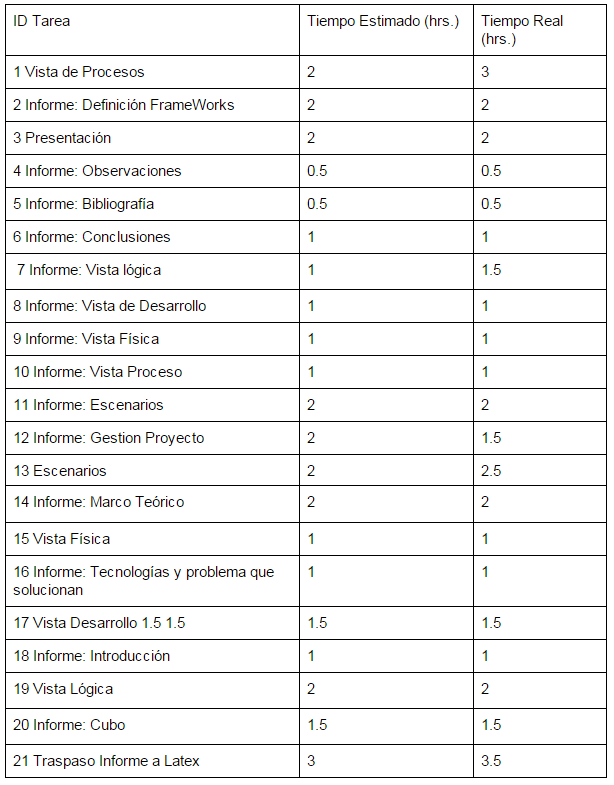
\includegraphics[width=15cm]{estimacionTareas1.png}
}


Ahora la cantidad de horas de trabajos estimadas son 31 hrs, Las horas de trabajo real fueron 33 hrs , notar que las horas reales trabajadas superaron las horas estimadas en 2 hrs aprox, esto quiere decir que las tareas se estimaron correctamente en su mayoría, ya que este margen de error fue relativamente bajo. Tiempo promedio por tarea fue de 1.48 hrs. Otros datos que se obtiene al analizar lo anterior son:

\begin{itemize}
	\item Estimación Trabajo Diario Grupo: 7.5 
	\item Horas Disponibles en Sprint por cada integrante: 37.5 
	\item Horas Disponibles en Sprint del Grupo: 187.5 
	\item Trabajo por dia promedio ideal 2.59 
\end{itemize}

Cabe señalar que si se trabajara de manera ideal, sobraría  tiempo equivalente a $187.5hrs - 31hrs = 156,5hrs$. 

A continuación se presentan los gráficos BurnDown y BurnUP con el fin de señalar la forma en que se trabajó a lo largo del Sprint.

\figura{Gráfico Burnup}{
	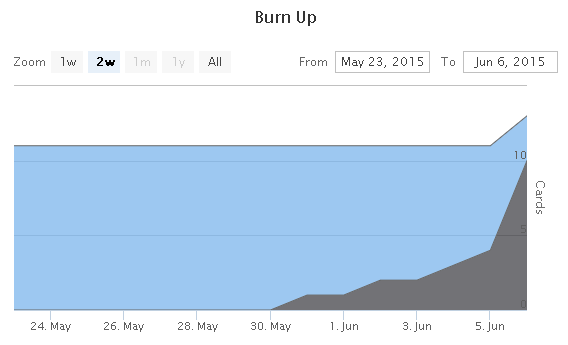
\includegraphics[width=15cm]{burnUp.png}
}

\newpage
\figura{Gráfico BurnDown}{
	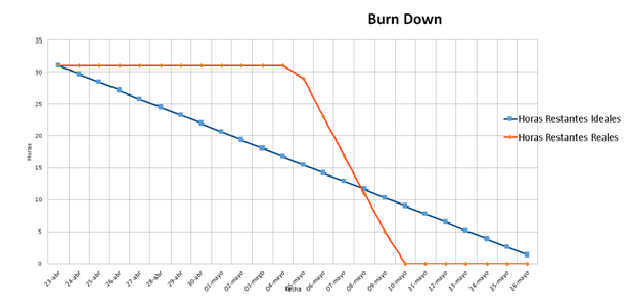
\includegraphics[width=15cm]{burnDown.png}
}

Como se aprecia en la imagen, se observa que en determinados periodos se trabajó una mayor cantidad, si bien alcanzamos a realizar la mitad del trabajo estimado a la fecha 8 de Mayo, se comenzó a trabajar en el proyecto varios días después de la planificación del \textsl{sprint}, por estos motivos se le solicitó al profesor mover la fecha de evaluación de la entrega de diseño arquitectural. Luego desde el 6 al 12 de mayo se comenzó a trabajar con gran rapidez, como se aprecia se terminó de ocupar las otras disponibles el 11 de mayo, el resto de los días si bien se trabajo, pero se trabajo tiempo superior al estimado.

Cabe destacar que para la próxima entrega se estimaron las tareas con \textsl{PokerPlaning} y se utilizará otra plataforma para realizar un análisis de datos, denominada \textsl{OllertApp}, la que facilitará el análisis de manera directa con lo realizado en \textsl{Trello}.

%-------------------------------------------------------------------------------------
\capitulo{OBSERVACIONES.}

En esta ocasión no se indicaron observaciones pertinentes al contenido del informe, sino mas bien consejos y sugerencias con respecto a la planificación, organización y trabajo en equipo.

%-------------------------------------------------------------------------------------
\capitulonn{CONCLUSIONES.}

Para la plataforma \textsl{BitPhoto}, es esencial diseñar correctamente el proyecto desde sus etapas más tempranas, es por eso que el Diseño Arquitectural es vital para el desarrollo y despliegue posterior de la aplicación.

El modelo 4+1 vistas y el Cubo 3D Suntone ayudan enormemente a llevar la visión de los arquitectos de software hacia los programadores, diseñadores y demás \textsl{stakeholders} de la aplicacion. En el contexto de la Ingeniería de Software resulta esencial comunicar correctamente la conceptualización de las ideas dentro del equipo de trabajo, para evitar inconsistencias en el producto final.

En esta entrega también se definen las tecnologías y sus versiones respectivas a utilizar dentro de la plataforma. Una clara definición del software y hardware que forman la plataforma condiciona la forma de trabajo, pero a la vez permite que los desarrolladores exploten de mejor manera los recursos tecnológicos disponibles.

Como siempre, la metodología ágil del proyecto implica constante comunicación entre los miembros del equipo desarrollador de \textsl{BitPhoto}. Llevando un control de las tareas desarrolladas se permite vigilar las cargas de trabajo.

Finalmente, se puede concluir que la plataforma \textsl{BitPhoto} pasó la etapa de Diseño Arquitectural, para iniciar posteriormente la etapa de Diseño Detallado. Los errores metodológicos a la hora de generar los esquemas y diagramas fueron debidamente corregidos.


%-------------------------------------------------------------------------------------

\capitulonn{BIBLIOGRAFÍA.}

[1] Philippe Kruchten. (Noviembre, 1995). En Planos Arquitectónicos: : El Modelo de “4+1” Vistas de la Arquitectura del Software(16). IEEE Software. 

Sitio Web: http://cic.puj.edu.co/wiki/lib/exe/fetch.php?media=materias:modelo4\_1.pdf

[2] SUNTONE ARCHITECTURE METHODOLOGY A 3-DIMENSIONAL APPROACH TO ARCHITECTURAL DESIGN. 11-Mayo-2015, de Sun MicroSystems 

Sitio web: http://rieck.dyndns.org/architecture/suntoneam\_wp\_5.24.pdf?version=1



\end{document}